\documentclass[11pt,a4paper]{article}
\usepackage[margin=2.3cm]{geometry}
\usepackage[T1]{fontenc}
\usepackage{lmodern}
\usepackage{amsmath,amssymb}
\usepackage{booktabs}
\usepackage{array}
\usepackage[dvipsnames]{xcolor}
\usepackage{tikz}
\usetikzlibrary{positioning,arrows.meta}
\usepackage[colorlinks=true,linkcolor=MidnightBlue,urlcolor=MidnightBlue]{hyperref}

\setlength{\parskip}{0.55em}
\setlength{\parindent}{0pt}

% Coloured boxes with plain xcolor (BasicTeX has no tcolorbox)
\newsavebox{\boxcontent}
\newcommand{\boxopen}[1]{\begin{lrbox}{\boxcontent}\begin{minipage}{\dimexpr\linewidth-14pt-0.8pt\relax}\setlength{\parskip}{0.4em}{\bfseries #1}\par}
\newenvironment{idea}[1]{\boxopen{#1}}{\end{minipage}\end{lrbox}\par\medskip\noindent{\setlength{\fboxsep}{7pt}\fcolorbox{MidnightBlue!60}{MidnightBlue!5}{\usebox{\boxcontent}}}\par\medskip}
\newenvironment{example}[1]{\boxopen{#1}}{\end{minipage}\end{lrbox}\par\medskip\noindent{\setlength{\fboxsep}{7pt}\fcolorbox{ForestGreen!60}{ForestGreen!5}{\usebox{\boxcontent}}}\par\medskip}
\newenvironment{caveat}[1]{\boxopen{#1}}{\end{minipage}\end{lrbox}\par\medskip\noindent{\setlength{\fboxsep}{7pt}\fcolorbox{BrickRed!55}{BrickRed!4}{\usebox{\boxcontent}}}\par\medskip}

\title{\textbf{How the Beyond-the-Clinic relapse monitor works}\\[0.3em]
\large A plain-language guide to the model, with the maths kept simple}
\author{Junction 2026 -- Aalto challenge team}
\date{14 November 2026 \quad (matches branch \texttt{relapse-hmm}, PR \#17)}

\begin{document}
\maketitle

\begin{idea}{The idea in four sentences}
We do \textbf{not} diagnose depression. We start when a patient is well after TMS treatment and learn
what their \emph{own healthy normal} looks like. Every day we measure how far today is from that normal,
in the direction that depressed voices and diaries typically move. If the patient stays clearly on the
``worse'' side for several days, friends get a gentle nudge and then the clinician is alerted.
\end{idea}

\tableofcontents
\vspace{0.5em}

% ------------------------------------------------------------------------------------------
\section{The whole pipeline at a glance}

\begin{center}
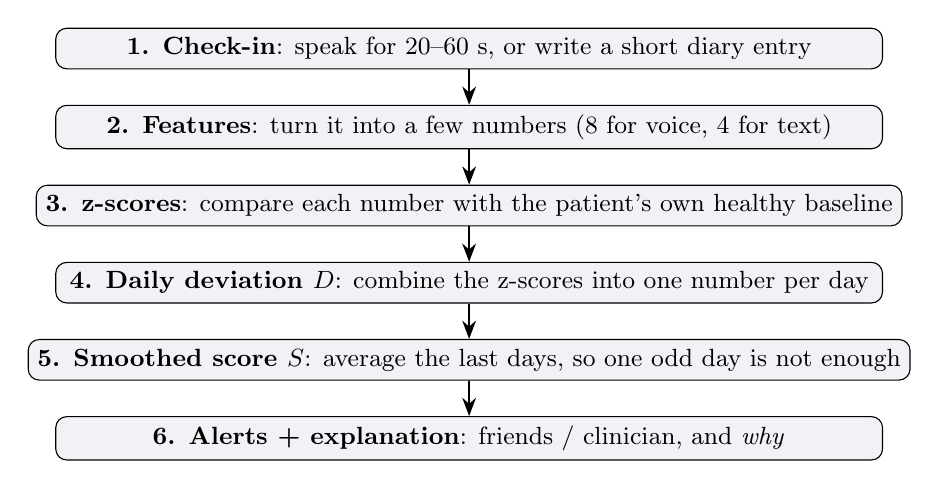
\begin{tikzpicture}[node distance=0.45cm, every node/.style={draw, rounded corners, fill=MidnightBlue!6, align=center, minimum width=10.5cm, font=\small}]
\node (a) {\textbf{1. Check-in}: speak for 20--60 s, or write a short diary entry};
\node (b) [below=of a] {\textbf{2. Features}: turn it into a few numbers (8 for voice, 4 for text)};
\node (c) [below=of b] {\textbf{3. z-scores}: compare each number with the patient's own healthy baseline};
\node (d) [below=of c] {\textbf{4. Daily deviation $D$}: combine the z-scores into one number per day};
\node (e) [below=of d] {\textbf{5. Smoothed score $S$}: average the last days, so one odd day is not enough};
\node (f) [below=of e] {\textbf{6. Alerts + explanation}: friends / clinician, and \emph{why}};
\foreach \x/\y in {a/b,b/c,c/d,d/e,e/f} \draw[-{Stealth}, thick] (\x) -- (\y);
\end{tikzpicture}
\end{center}

There are three \emph{branches} that feed step 4: \textbf{acoustic} (the voice), \textbf{text}
(a written diary, or the transcript of a spoken check-in) and, later, \textbf{health} (wearable data).
This guide uses the acoustic branch as the running example; the text branch works the same way from
step 3 on.

% ------------------------------------------------------------------------------------------
\section{Step 1--2: from a recording to eight numbers}

Two off-the-shelf tools turn the audio into numbers. \textbf{Neither is trained by us.}

\begin{center}
\small
\begin{tabular}{@{}llp{6.6cm}@{}}
\toprule
\textbf{Feature} & \textbf{Tool} & \textbf{What it measures (``worse'' direction)} \\
\midrule
\texttt{speech\_rate} & openSMILE & voiced segments per second $\approx$ syllables per second (\emph{lower})\\
\texttt{f0\_std}      & openSMILE & how much the pitch varies -- monotone voice (\emph{lower})\\
\texttt{pause\_ratio} & openSMILE & share of unvoiced time, i.e. pauses (\emph{higher})\\
\texttt{energy}       & openSMILE & loudness (\emph{lower})\\
\texttt{jitter}       & openSMILE & small irregularities in pitch (\emph{higher})\\
\texttt{shimmer}      & openSMILE & small irregularities in loudness (\emph{higher})\\
\texttt{arousal}      & wav2vec2  & how energetic the voice \emph{sounds} (\emph{lower})\\
\texttt{valence}      & wav2vec2  & how positive the voice \emph{sounds} (\emph{lower})\\
\bottomrule
\end{tabular}
\end{center}

openSMILE cuts the sound into short windows (about 20--60 ms), runs a Fourier transform on each to get
its frequencies, measures pitch and loudness, and then averages over the whole recording.
wav2vec2 is a neural network that listens to the raw sound wave and outputs ``arousal'' and ``valence''
between 0 and 1. The text branch similarly gives 4 numbers (e.g.\ how close the wording is to depression
on a model trained on Reddit, and the sentiment).

% ------------------------------------------------------------------------------------------
\section{What we learn from the Androids Corpus (and what we do not)}

The Androids Corpus has interview recordings of \textbf{114 different people}: 62 diagnosed with
depression and 52 healthy controls. \textbf{Each person was recorded once.} Nobody appears both
depressed and well. Each interview is cut into short clips (median 6 clips per person), all from the
same conversation.

From it we learn three things:
\begin{enumerate}
\item \textbf{Do the features carry a depression signal at all?} A simple classifier that only sees the
8 numbers tells depressed from healthy people it has never seen with an \textbf{AUC of 0.77}.
(AUC = the chance that a random depressed person gets a higher score than a random healthy person;
0.5 = guessing, 1.0 = perfect.) Gender and age alone give 0.48, so it is not just demographics.
\item \textbf{In which direction does each feature move?} For all 8 features the direction matches the
research literature (column ``worse'' in the table above).
\item \textbf{How much does one person's voice wobble between clips, and which features wobble
together?} Because every person has several clips, we can measure the \emph{within-person spread}
of each feature and how strongly pairs of features move together (e.g.\ arousal and energy: 0.59).
\end{enumerate}

\begin{caveat}{What the corpus cannot tell us}
How a \emph{single person's} voice changes when they relapse. The corpus compares \emph{different}
people. We \textbf{assume} that a relapse moves a person in the same direction as the difference
between depressed and healthy people. That is plausible and supported by the literature, but untested.
\end{caveat}

% ------------------------------------------------------------------------------------------
\section{Step 3: the healthy baseline}

During the first \textbf{14 days after treatment} (at least 10 check-ins) the app only collects. Then it
\emph{locks} a baseline, separately for morning and evening. For every feature it stores two numbers:

\textbf{Centre} $c$ = the \emph{median} of the baseline values (the middle value; one strange day does
not move it).

\textbf{Spread} $\sigma$ = how much this feature normally wobbles for this person. With only 14--28
values a personal spread is uncertain, so we mix it with the spread measured in the corpus:
\[
\sigma^2 \;=\; \frac{n\cdot s_{\text{personal}}^2 \;+\; 5\cdot s_{\text{corpus}}^2}{n+5}
\]
\begin{itemize}
\item $n$ = number of baseline values, $s_{\text{personal}}$ = the person's own spread (computed robustly from
the median distance to the median, ``MAD'').
\item $s_{\text{corpus}}$ = the typical within-person spread from the Androids Corpus.
\item With few values the corpus dominates; with many values the person's own data takes over.
\end{itemize}

The baseline is \textbf{never updated automatically}: otherwise a slow relapse would slowly become the
``new normal'' (the boiling-frog problem). Only the clinician can start a new one.

% ------------------------------------------------------------------------------------------
\section{Step 3 continued: the z-score -- ``how unusual is today?''}

For each feature:
\[
z \;=\; \text{direction}\times\frac{x - c}{\sigma}
\qquad\text{(direction} = +1 \text{ if higher is worse, } -1 \text{ if lower is worse)}
\]
$z$ answers: ``how many of my usual wobbles am I away from my healthy normal, and is it in the worse
direction?'' \textbf{Positive $z$ = worse}, negative $z$ = better than normal.

\begin{example}{Worked example: arousal in one ``bad'' recording}
Baseline centre $c = 0.473$, spread $\sigma = 0.063$, today $x = 0.308$, and lower arousal is worse
(direction $=-1$):
\[
z = -1\times\frac{0.308-0.473}{0.063} = +2.6
\]
Today's voice sounds 2.6 ``normal wobbles'' less energetic than this person's healthy normal.
\end{example}

% ------------------------------------------------------------------------------------------
\section{Step 4: the daily deviation $D$ -- one number per day}

We combine the eight z-scores into one number. Every feature counts equally ($w = 0.125$):
\[
D \;=\; \frac{w_1 z_1 + w_2 z_2 + \dots + w_8 z_8}{\text{normal wobble of that sum}}
\]
The bottom line makes $D$ have the same scale every day: \textbf{when nothing has changed, $D$ wobbles
around 0 with a standard deviation of 1.} So ``$D = 2$'' always means ``twice the normal wobble''.

\textbf{Why the bottom line is not simple.} Some features move together (arousal and energy correlate
0.59 within a person). If two features always moved together, counting both would just count the same
wobble twice, and the sum would wobble more than if they were independent. The bottom line takes this
into account using the correlations measured in the corpus. For our 8 features it is $0.450$ (it would
be $0.354$ if they were independent).

\begin{example}{Worked example: the same recording, all 8 features}
\small
\begin{tabular}{@{}lrrrrrrrr@{}}
\toprule
 & arousal & valence & energy & speech & pauses & jitter & shimmer & pitch var.\\
\midrule
$z$ & $+2.63$ & $+2.60$ & $+0.97$ & $+0.49$ & $+0.32$ & $-1.10$ & $-1.18$ & $-1.55$\\
\bottomrule
\end{tabular}
\[
D = \frac{0.125\times(2.63+2.60+0.97+0.49+0.32-1.10-1.18-1.55)}{0.450} = \frac{0.396}{0.450} = 0.88
\]
The voice sounded flatter and more negative, but pitch irregularities moved the other way, so the
day is only mildly unusual ($D=0.88$ happens on roughly 1 in 5 ordinary days).
\end{example}

\textbf{Two branches on the same day} (voice and diary): we take the average of their $D$ values.

% ------------------------------------------------------------------------------------------
\section{Step 4 continued: several check-ins on the same day}

If a patient checks in twice a day (morning and evening), we combine the two $D$ values of a branch as
\[
D_{\text{day}} \;=\; \frac{D_{\text{morning}} + D_{\text{evening}}}{\sqrt{2}}
\]
\begin{itemize}
\item The \textbf{noise} still has standard deviation 1 (two independent wobbles of size 1, added and divided by $\sqrt2$).
\item A \textbf{real change} that shows up in both check-ins grows by a factor $\sqrt2\approx1.41$.
\end{itemize}
So two check-ins a day make a real change easier to see without causing more false alarms. In the
simulator this \textbf{roughly halves the number of missed relapses} (Section~\ref{sec:howgood}).

% ------------------------------------------------------------------------------------------
\section{Step 5: the smoothed score $S$}

One bad day is not a relapse. We therefore average the recent days, giving most weight to today:
\[
S_{\text{today}} \;=\; 0.3\cdot D_{\text{today}} \;+\; 0.7\cdot S_{\text{yesterday}}
\]
Unrolled, this is a weighted average of the last days:

\begin{center}
\small
\begin{tabular}{@{}lcccccc@{}}
\toprule
Day & today & yesterday & 2 days ago & 3 days ago & 4 days ago & \dots\\
\midrule
Weight & 0.30 & 0.21 & 0.147 & 0.103 & 0.072 & \dots\\
\bottomrule
\end{tabular}
\end{center}

We compute $S$ twice:
\begin{itemize}
\item $S_{\text{anchored}}$: against the \textbf{healthy baseline}. This catches \emph{slow drift}.
\item $S_{\text{rolling}}$: against the \textbf{last 14 days}. This catches \emph{abrupt change}.
\end{itemize}
The app uses the \textbf{higher of the two}, and tells the clinician which one it was.

% ------------------------------------------------------------------------------------------
\section{Step 6: alerts}

\begin{center}
\small
\begin{tabular}{@{}>{\raggedright\arraybackslash}p{4.2cm}>{\raggedright\arraybackslash}p{5.0cm}>{\raggedright\arraybackslash}p{5.2cm}@{}}
\toprule
\textbf{Who} & \textbf{When} & \textbf{False alerts per healthy patient-year (simulated)}\\
\midrule
Friends (a hint, no health data) & $S>1$ for 3 days in a row & 2.3 -- 4.8 (target $\le 2$: open issue)\\
Clinician & $S>2$, or $S>1$ for 7 days & 0.4 -- 1.4\\
Clinician, immediately & crisis phrases in the text/transcript & --\\
Clinician only (``elevated'') & $S_{\text{anchored}}<-1$ for 3 days & $\approx$1 -- 1.9\\
\bottomrule
\end{tabular}
\end{center}

The thresholds 1 and 2 were \emph{chosen}, not fitted. Because $D$ has standard deviation 1 under
``no change'', they mean ``one/two normal wobbles''. The simulator shows what they cost in false alarms
(right column). The \textbf{elevated} flag catches unusually \emph{good} streaks, which can be a warning
sign too (hypomania in bipolar patients); it goes to the clinician only, never to friends.

% ------------------------------------------------------------------------------------------
\section{Step 6 continued: the explanation -- nothing is hidden}

Both formulas above are plain sums, so the score splits exactly:
\[
S = \underbrace{0.30\cdot D_{\text{today}} + 0.21\cdot D_{\text{yesterday}} + \dots}_{\text{which days}}
\qquad\text{and}\qquad
D = \underbrace{\text{share}_{\text{arousal}} + \text{share}_{\text{energy}} + \dots}_{\text{which features}}
\]
with $\text{share}_i = w_i z_i / 0.450$. The clinician therefore sees, for example:
\emph{``$S = 2.72$: diary language closer to depression $+2.03$, more negative wording $+0.34$,
less steady pitch $+0.19$, \dots''} and the sentence \emph{``Compared with the healthy normal over the
last days: diary language closer to depression and more negative wording.''}

% ------------------------------------------------------------------------------------------
\section{``Typical shift with depression'' -- what it is, and how much it matters}
\label{sec:shift}

\begin{idea}{Definition in one line}
For each feature: how far apart are the \emph{average depressed person} and the \emph{average healthy
person}, measured in units of \emph{one person's normal wobble}?
\[
\delta \;=\; \frac{\text{average of depressed people} \;-\; \text{average of healthy people}}{\text{normal within-person wobble}}
\]
\end{idea}

\begin{example}{Worked example: arousal}
\begin{enumerate}
\item Average arousal of the 52 healthy speakers: $0.413$. Of the 62 depressed speakers: $0.308$.
      Difference: $0.308-0.413 = -0.105$.
\item ``Normal within-person wobble'': for each speaker, look at how their own clips spread around
      their own average, and pool this over all speakers. For arousal this is $0.0743$.
      (One depressed speaker's five clips, for illustration: 0.175, 0.140, 0.295, 0.048, 0.193 --
      the same person, the same conversation, and still quite a spread.)
\item $\delta = -0.105 / 0.0743 = \mathbf{-1.42}$.
\end{enumerate}
In words: \emph{if a person went from sounding like the average healthy speaker to sounding like the
average depressed speaker, their arousal would drop by about 1.4 of their own normal day-to-day
wobbles.} That is large enough to notice over a few days, but not on a single day.
\end{example}

\begin{center}
\small
\begin{tabular}{@{}lrrrrrrrr@{}}
\toprule
 & arousal & energy & valence & jitter & pauses & speech & shimmer & pitch var.\\
\midrule
$\delta$ (worse direction) & 1.42 & 1.19 & 0.88 & 0.54 & 0.44 & 0.30 & 0.28 & 0.24\\
Share of $D$ in a full relapse & 27\% & 23\% & 17\% & 10\% & 8\% & 6\% & 5\% & 5\%\\
\bottomrule
\end{tabular}
\end{center}

\textbf{How important is it for the model?}
\begin{itemize}
\item \textbf{Not needed to compute a score.} The app uses equal weights; $\delta$ does not enter the
      formula for $D$ or $S$.
\item \textbf{Useful to understand the score.} With equal weights, the features that shift most
      ($\delta$ large) automatically drive the score: arousal, energy and valence give about two thirds
      of the signal in a relapse (bottom row).
\item \textbf{Used in the simulator} to create realistic synthetic relapses, and it tells us how big a
      signal to expect: a full relapse moves $D$ by about \textbf{1.5} (measured on held-out speakers).
\end{itemize}

\begin{caveat}{Why we did not use $\delta$ to set the weights}
We tried weighting features by $\delta$ (and three other ways). On speakers the method had not seen,
all four gave the same result within noise (1.54 -- 1.61, while the five test groups ranged 0.8 -- 3.1).
With 114 people the data cannot justify finer weights, so we use the simplest: equal weights.
\end{caveat}

% ------------------------------------------------------------------------------------------
\section{How good is it?}
\label{sec:howgood}

We cannot test relapse detection on real patients yet (that needs months of data). Instead a
\textbf{simulator} creates synthetic patients: their voice features are drawn from the corpus
statistics, a slow relapse starts on day 40 and builds over about 15 days, and \emph{the real app
code} scores every day. ``Noise $\times1.5$'' means real day-to-day wobble is 1.5 times the
within-conversation wobble measured in the corpus (we do not know the true value yet).

\begin{center}
\small
\begin{tabular}{@{}lcc@{}}
\toprule
\textbf{Day-to-day noise} & \textbf{Missed relapses of 100, 1 check-in/day} & \textbf{2 check-ins/day}\\
\midrule
$\times1.0$ & 24 & 6\\
$\times1.5$ & 40 & 18\\
$\times2.0$ & 46 & 32\\
\bottomrule
\end{tabular}
\end{center}

\textbf{We also tried a more advanced model} (a hidden Markov model that outputs a probability of
relapse). At the same number of false alarms it detected the same relapses, and its probabilities were
over-confident. We kept the simpler, fully explainable rule.

\begin{caveat}{The real bottleneck}
A baseline from only 14 check-ins has a small, \emph{permanent} error: for some healthy patients $D$
sits around $+0.5$ for ever, for others around $-0.5$. No alert rule can fix that. What helps:
two check-ins a day, a longer baseline, more branches (diary, wearable), and measuring real
day-to-day noise.
\end{caveat}

% ------------------------------------------------------------------------------------------
\section{Assumptions and limits -- said plainly}
\begin{enumerate}
\item A relapse moves a person in the direction that separates depressed from healthy people
      (between-person data used for within-person change).
\item Real day-to-day noise is unknown; the corpus only shows wobble within one conversation.
\item Loudness (\texttt{energy}) depends on the microphone and the distance to the phone.
\item The corpus is Italian; prosody transfers reasonably, content is handled by the text branch.
\item The alert thresholds are chosen and then checked in simulation, not learned from patients.
\item Validation of real relapse detection needs a longitudinal clinical pilot (e.g.\ with PHQ-9).
\end{enumerate}

\textbf{What we can honestly say:} \emph{``We measure deviation from the patient's own healthy normal,
in a direction validated on a clinical corpus. Alert thresholds are checked against a false-alarm target
in simulation. Whether it detects relapse must be validated in a clinical pilot.''}

% ------------------------------------------------------------------------------------------
\section*{Glossary}
\begin{description}
\item[Median] the middle value when sorted; robust to one extreme value.
\item[Standard deviation (SD)] the typical size of a wobble around the average.
\item[MAD] median absolute deviation: the median distance from the median; $1.48\times$MAD $\approx$ SD.
\item[Within-person vs between-person] wobble of \emph{one} person over time vs differences \emph{between} people.
\item[z-score] distance from the centre, in units of the normal wobble.
\item[Correlation] how much two features move together (0 = not at all, 1 = always).
\item[EWMA] exponentially weighted moving average -- the smoothing in Step 5.
\item[AUC] chance that a random depressed person scores higher than a random healthy one (0.5 = guessing).
\item[Held-out] tested on people the method was not fitted on.
\end{description}

\end{document}
